\documentclass[border=10pt]{standalone}

\usepackage{tikz}
\usepackage{tikzsymbols}
\usetikzlibrary{calc,patterns,shapes.geometric}

\def\centerarc[#1](#2)(#3:#4:#5){\draw[#1] ($(#2)+({#5*cos(#3)},{#5*sin(#3)})$) arc (#3:#4:#5);}

\begin{document}
	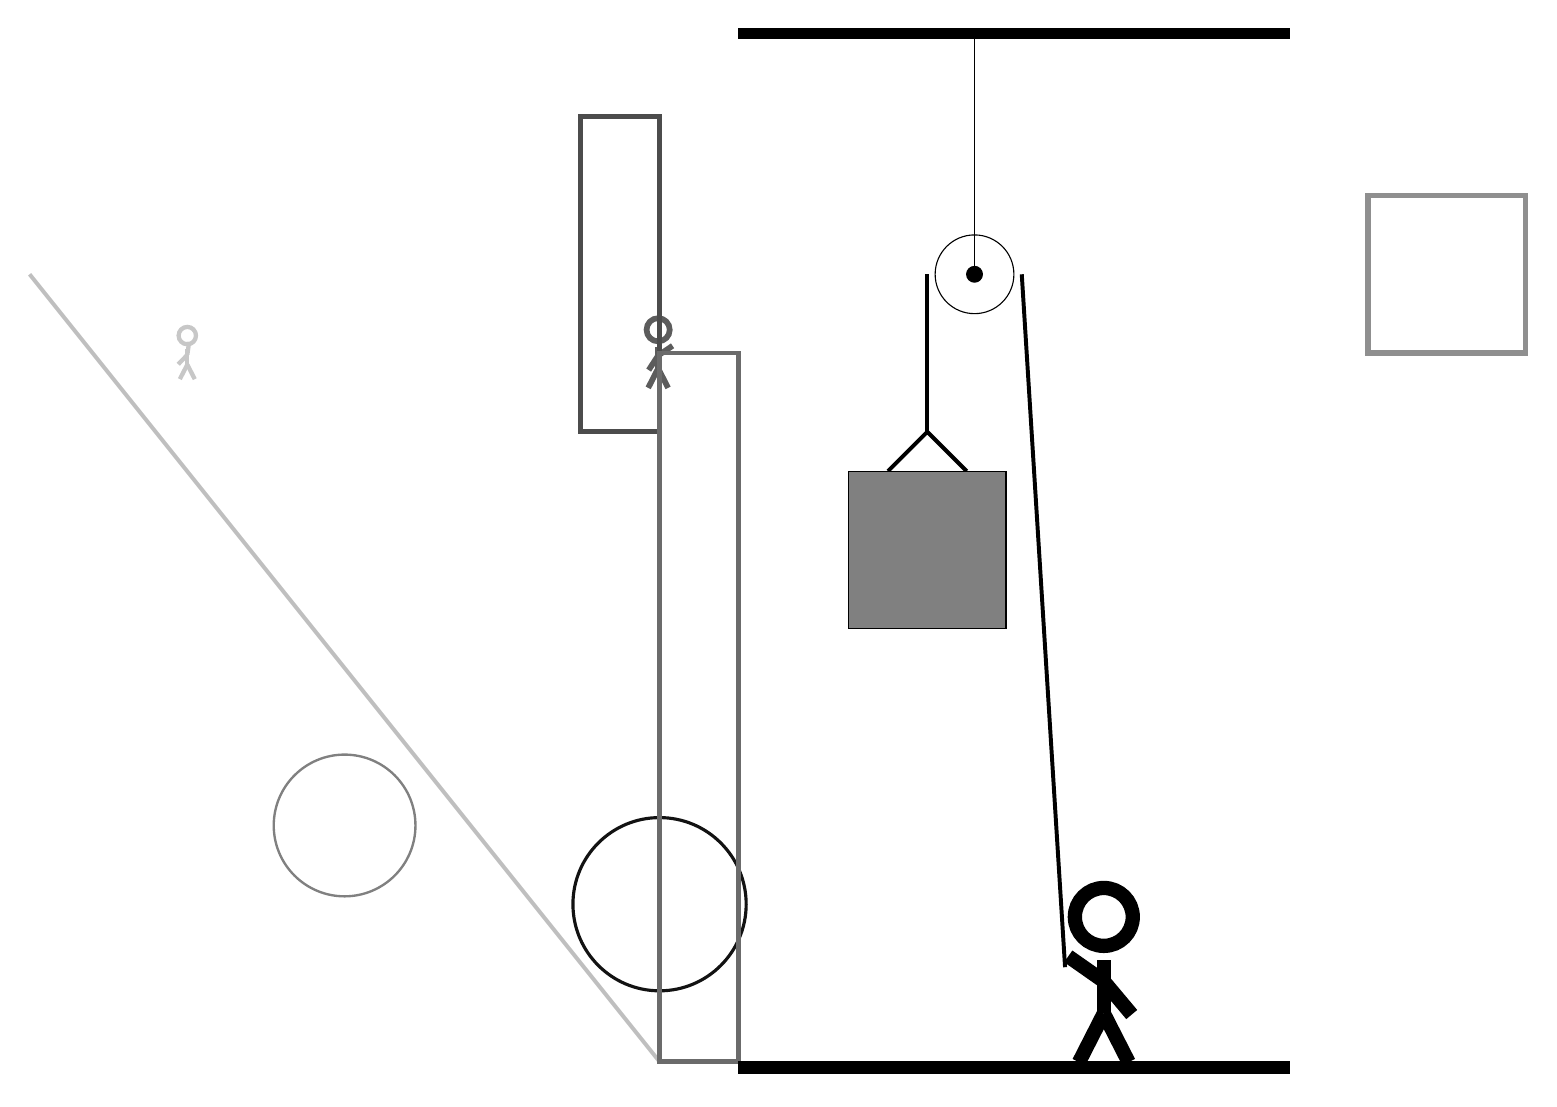
\begin{tikzpicture}
		%%%%% START %%%%%
		
		\draw[fill=black] (-2, 10) rectangle (5, 10.125);
		
		\draw (1, 7) circle (0.5);
		\draw[fill=black] (1, 7) circle (0.1);
		\draw (1, 10) -- (1, 7);
		
		\draw[line width=0.5mm] (-0.1, 4.5) -- (0.4, 5.0) -- (0.9, 4.5);
		\draw[fill=black!50] (-0.6, 4.5) rectangle (1.4, 2.5);
		
		\draw[line width=0.5mm] (0.4, 7) -- (0.4, 5.0);
		\centerarc[line width=0.5mm](1, 7)(0:180:0.6);
		\draw[line width=0.5mm](1.6, 7) -- (2.15, -1.8);
		
		\node at (2.6, -1.9) {\Strichmaxerl[10][-35][-50]};
		
		\draw[line width=0.5mm, color=black!25](-3, -3) -- (-11, 7);
		
		\node[line width=0.4mm, color=black!64] at (-3, 6) {\Strichmaxerl[4][57][34]};
		\draw[line width=0.6mm, color=black!70] (-3, 9) rectangle (-4, 5);
		\draw [line width=0.4mm, color=black!93](-3, -1) circle (1.1);
		\draw[line width=0.6mm, color=black!58] (-2, 6) rectangle (-3, -3);
		
		\draw [line width=0.3mm, color=black!50](-7, 0) circle (0.9);
		
		\node[line width=0.6mm, color=black!22] at (-9, 6) {\Strichmaxerl[3][46][82]};
		\draw[line width=0.7mm, color=black!44] (6, 6) rectangle (8, 8);
		
		\draw[fill=black] (-2, -3) rectangle (5, -3.15);
		
		%%%%% END %%%%%
	\end{tikzpicture}
\end{document}